\section{Problem Statement} \label{sec:problemstatement} 
There are two main problems: one has something to do with the developing process and the other is complex product-oriented challenge.

\textbf{First:} problems with most (if not all) other Linux distributions are due to bad documenting. 

\textbf{Second:} Linux distributions may consist of hundreds of packages and these packages may have dozens of dependencies. Finding a way in this jungle of dependencies is a serious problem in an SPMS. All kinds of dependencies must be taken into account. For example, if a package manager only deals with build time dependencies then a software package can be installed and compiled. A problem pops up when one runs into  run time dependencies, which are needed for starting and running the program. Another core problem is sorting a list of software packages to build in an order such that the minimum number of rebuilds are achieved. When a program has to be installed, re-installed, or reconfigured, it may have an affect on some other package(s).

\textbf{Running example:} the graph in Figure \ref{fig:example} shows our running example dependency tree which will be used throughout the rest of this document.

\begin{figure}
	\centering
	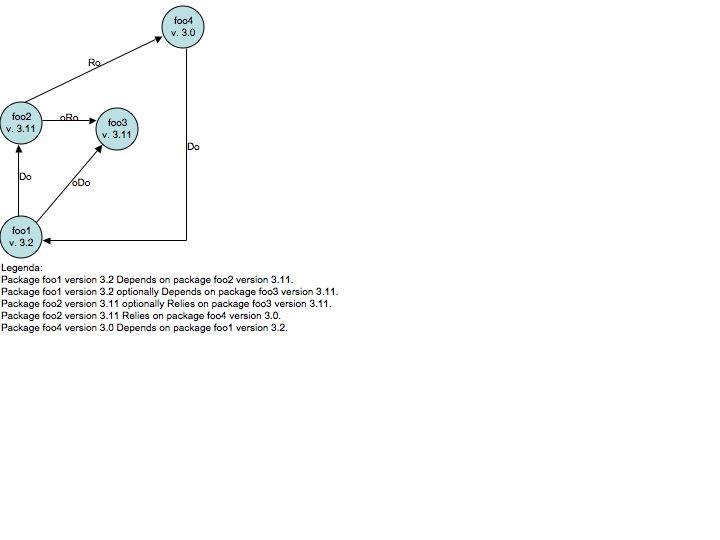
\includegraphics[bb=0 0 720 540]{problem/Slide1.jpg}
% Slide1.jpg: 300dpi, width=6.10cm, height=4.57cm, bb=0 0 720 540
	\caption{Example software package dependency tree}
	\label{fig:example}
\end{figure}
